\documentclass{gapd}

\Type{Short Note}
\Title{Uniqueness in Logic Puzzles}

\Author{James Tiberius Kirk}{NCC~1701, Enterprise}

\Author{Montgomery Scott}{NCC~1701, Enterprise}

\Author{Leonard McCoy}{NCC~1701, Enterprise}

\Abstract{Pure deduction puzzles typically have a single unique
  solution.  However, some puzzle setters argue that challenges with
  multiple solutions are also valid, if they can be solved by
  eliminating choices that lead to ambiguous states.  This paper
  considers the arguments for and against this position, and presents
  a counterexample that demonstrates the danger of using uniqueness to
  decide between multiple solutions.}

\Issue{1}{1}{2015}
%\Pages{35}{37}

\begin{document}
\maketitle

\section{Introduction}
\label{sec:Introduction}

\lettrine{A}{} characteristic of pure deduction puzzles,
such as Japanese logic puzzles, is that each challenge has a single
unique solution.  This allows such challenges to be solved by
deduction rather than guesswork~\cite{browne}.

I was therefore surprised to find a Kakuro challenge with multiple
solutions in a publication as respectable as \textit{The
  Guardian}~\cite{guardian}.  This was the first time that I had ever
encountered such a case in print.  The aim in Kakuro is to fill each
cell with a digit in the range {\sf 1--9}, such that each horizontal
and vertical run adds to the hint total shown, and no digit is
repeated within each run~\cite{nikoli}.

Figure~\ref{fig:Kakuro} shows the relevant section of the Kakuro
challenge in question (all other values have been resolved).  Possible
values for the final few unresolved cells are shown in small print,
and a key cell with possible values {\sf 4} or {\sf 5} is circled.
This challenge has three possible solutions, depending on whether this
key cell takes the value {\sf 4} or {\sf 5}, as shown.

\begin{figure*}[!thb]
  \centering
  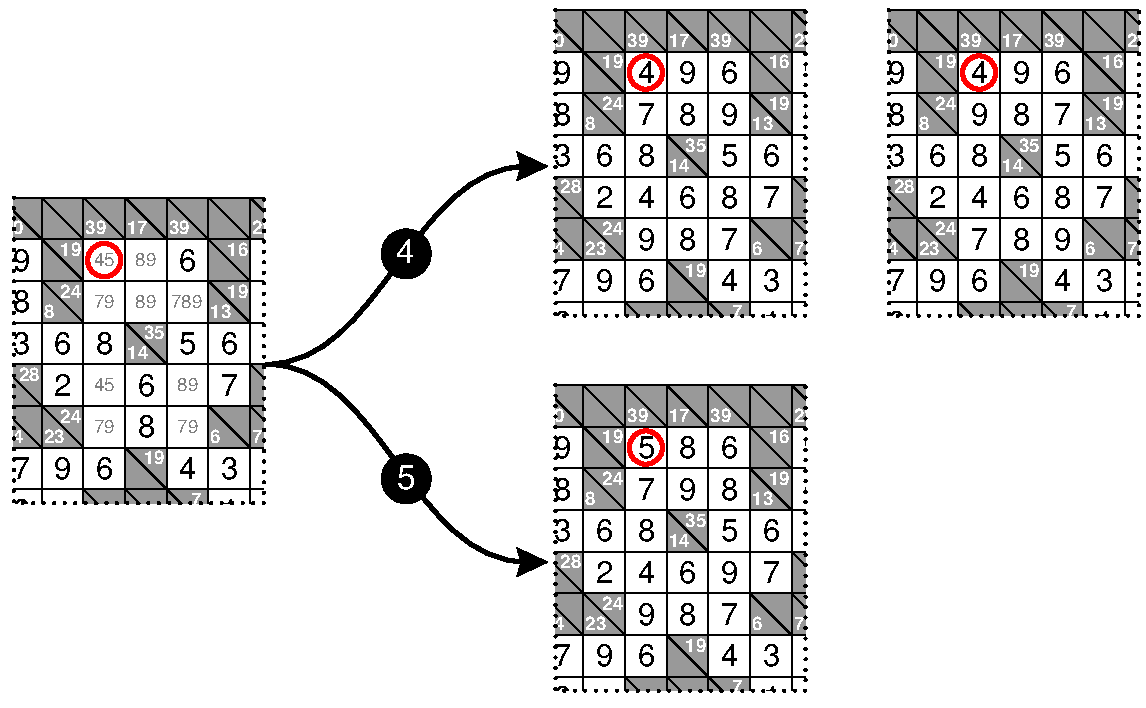
\includegraphics[width=\linewidth]{graphics/kakuro-1372-multiple-1.pdf}
  \caption{A Kakuro challenge with three solutions. The circled cell
    can take the value {\sf 4} or {\sf 5}.}
  \label{fig:Kakuro}
\end{figure*}

After alerting the UK setter of this challenge to what appeared to be
a flawed design with no deducible solution, I was also surprised by
his response.  He maintained that this challenge was indeed valid, and
could be solved by deduction based on \textit{relative} uniqueness.

\section{The Case For Ambiguity}
\label{sec:Ambiguity}

The setter of the ambiguous Kakuro challenge argued as follows:

\begin{quote}\itshape
  Any move M that leads to multiple solutions can be eliminated.
\end{quote}

For instance, the value of the circled cell in Figure~\ref{fig:Kakuro}
cannot be {\sf 4}, as such a move would allow multiple solutions (top
row).  This cell must therefore take the value {\sf 5}, producing the
single `correct' solution (bottom row).

This argument of \textit{deduction by relative uniqueness}, for selecting
among multiple solutions, seems fair enough at first glance.  It adds
some much-needed depth to Kakuro, by allowing an additional solution
strategy.  It also increases the number of possible challenges that
can be devised, by allowing cases with multiple solutions that
traditional setters would not allow.

However, Japanese publisher Nikoli, the inventor and major supplier of
Kakuro, categorically state that uniqueness should not be exploited in
this way to solve Kakuro, or any of their other pure deduction
puzzles.\footnote{Strongly worded personal correspondence.}  We now
consider the argument for absolute rather than relative uniqueness.

\section{The Case For Uniqueness}
\label{sec:Uniqueness}

A serious problem with deduction by relative uniqueness is that it
does not work unless the solver also knows that this rule is in force,
but uniqueness is generally assumed for such puzzles rather than
explicitly stated.  For example, the Kakuro rules provided by \textit{The
  Guardian} make no mention of uniqueness, making those rules
insufficient to solve the ambiguous challenge shown in
Figure~\ref{fig:Kakuro}~\cite{guardian}.

Further, there is an obvious corollary to the argument (1) made above:

\begin{quote}\itshape
  Any move leading to ambiguous move M can therefore also be
  eliminated.
\end{quote}

Hence, chaining backwards from ambiguous move $M$, every prior move
can also be said to lead to ambiguity and hence be eliminated, until
the challenge has no valid moves.  Or can it?  There is no clear
answer to this question, which depends on the setter's and solver's
interpretations.

\subsection{Counterexample}
\label{sec:Counteraxeample}

The following counterexample demonstrates the dangers of deduction by
relative uniqueness.  Slitherlink is a deduction puzzle in which a
simple closed path must be traced through orthogonal vertices of a
square grid, to visit the number of sides indicated on each numbered
cell~\cite{times}.  For example, Figure~\ref{fig:SlitherlinkSolutions}
shows a simple 2$\times$3 Slitherlink challenge with three valid
solutions: $a$, $b$ and $c$.

\begin{figure*}[!thb]
  \centering
  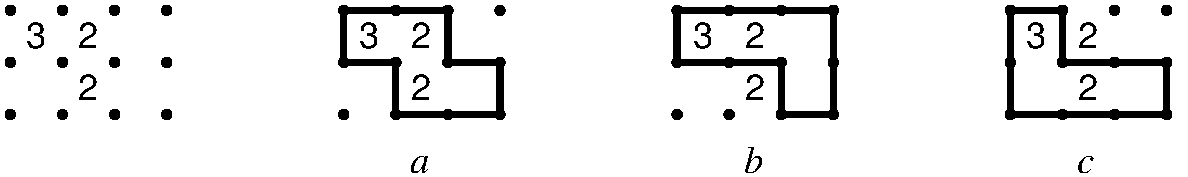
\includegraphics[width=\linewidth]{graphics/slitherlink-solns-1.pdf}
  \caption{A 2$\times$3
  Slitherlink challenge (left) with three solutions ($a$, $b$ and
  $c$).}
  \label{fig:SlitherlinkSolutions}
\end{figure*}

\begin{figure}[htb]
  \centering
  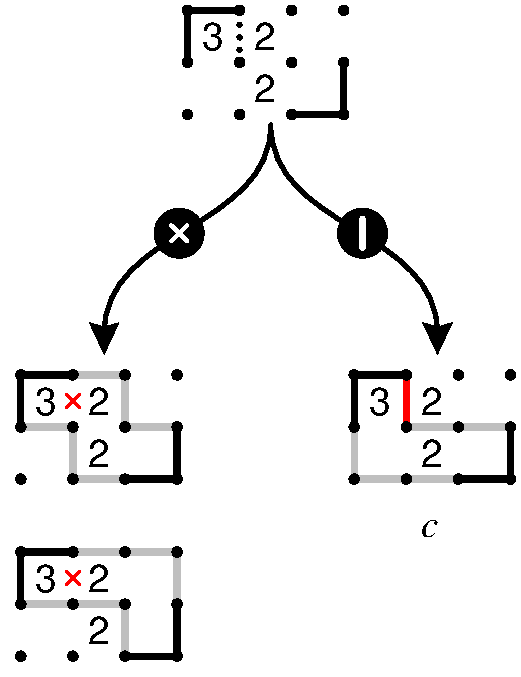
\includegraphics[width=0.85\columnwidth]{graphics/slitherlink-deduce-a2.pdf}
  \caption{Deduction by uniqueness yields $c$.}
  \label{fig:SlitherlinkDeductionA}
\end{figure}

Given that four edges can be deduced as shown in
Figure~\ref{fig:SlitherlinkDeductionA} (top), consider the move
indicated by the dotted line.  If there is \textit{not} an edge between
these vertices then two possible solutions exist (left), hence this
move must be an edge and $c$ must be the `correct' solution (right).

However, if the same process is applied to the move indicated in
Figure~\ref{fig:SlitherlinkDeductionB} (top, dotted), then $b$ is
deduced to be the `correct' solution (right).


\begin{figure}[htb]
  \centering
  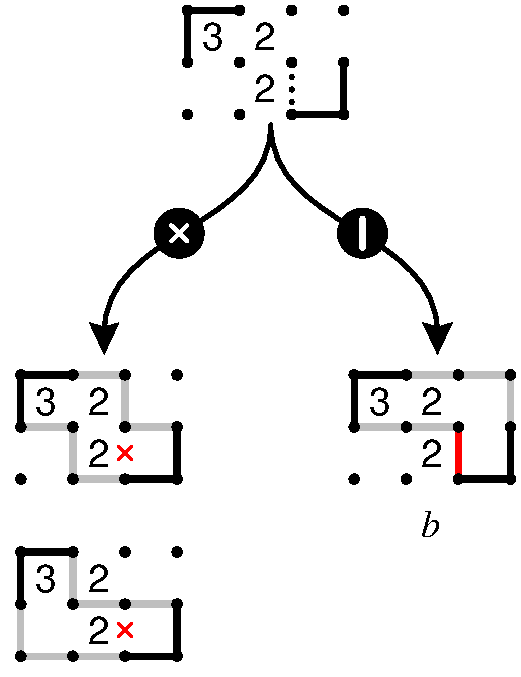
\includegraphics[width=0.85\columnwidth]{graphics/slitherlink-deduce-b2.pdf}
  \caption{Deduction by uniqueness yields $b$.}
  \label{fig:SlitherlinkDeductionB}
\end{figure}

Deduction by relative uniqueness therefore gives two conflicting
`correct' solutions, $b$ and $c$, depending on processing order.  To
derive the same solution as the setter, the solver would have to
follow the same sequence of decisions in the exact same order, but
there is no way to enforce this in practice.  Deduction by relative
uniqueness is not guaranteed to yield the same solution from among
multiple solutions in all cases.

This Slitherlink counterexample could be said to have one valid
solution (depending on the order in which the solver made their
deductions), two equally valid solutions (through deduction by
relative uniqueness) or three equally valid solutions (which it does,
after all---see Figure~\ref{fig:SlitherlinkSolutions}).  This is
clearly an unsatisfactory state of affairs.  But if absolute
uniqueness is enforced, and such cases of multiple solutions avoided,
then all of these problems simply go away, at no real cost.  As expert
puzzle designer Hiroshi Higashida points out:

\begin{quote}
  \textit{Puzzle creators, not only solvers, mustn't defy rules, either}
  \cite[p216]{Higashida2010}.
\end{quote}

\section{Conclusion}
\label{sec:Conclusion}

The characteristic of pure deduction puzzles to have a single unique
solution is not only elegant, but performs a vital practical function.
It guarantees that challenges can be solved by deduction alone,
without guesswork or ambiguity, and means that the setter and solver
are both playing from the same rule set without the need to make
assumptions about implied or hidden rules.  Further, uniqueness makes
challenges self-checking; if the player has deduced a solution, then
it must be the correct one.  As tempting as it may be to relax this
constraint of absolute uniqueness and instead exploit relative
uniqueness as a solution strategy, this is best avoided in pure
deduction puzzles.

\section*{Acknowledgements}

Thanks to Jimmy Goto for clarifying Nikoli's position on uniqueness.

\section*{References}

\begin{thebibliography}{4}

\bibitem{browne} Browne, C., `Deductive Search for Logic Puzzles',
  \textit{Computational Intelligence and Games (CIG'13)}, IEEE Press,
  2013, pp.~359--366.

\bibitem{guardian} Anonymous, `Kakuro', \textit{The Guardian},
  29~November~2013.

\bibitem{nikoli} \textit{Kakuro 1}, Tokyo, Nikoli, 1986.

\bibitem{times} \textit{The Times Japanese Logic Puzzles: Hitori, Hashi,
    Slitherlink and Mosaic}, London, Harper Collins, 2006.

\bibitem{Higashida2010} Higashida, H., `Machine-Made Puzzles and
  Hand-Made Puzzles', \textit{IFIP Advances in Information and
    Communication Technology (AICT)}, vol.~333, 2010, pp. 214--222.

\end{thebibliography}

\Note{BlueNoteBackground}{%
  {\bf Cameron Browne} is a Vice-Chancellor's Senior Research Fellow
  at QUT, Brisbane, Australia, whose research interests include artificial intelligence and automated game design.\\
  {\bf Address:} School of EECS, Science and Engineering Faculty, QUT,
  Brisbane, 4001, Australia.\\
  {\bf Email:} c.browne@qut.edu.au
%
}

\end{document}
